\newpage
\section{Anhang: Beispiele}
	\subsection{Ganze Zahl in String konvertieren (Array)} 
		Schreiben Sie ein Programm, das eine vorzeichenlose ganze Zahl einliest und diese 10 Zeichen breit (entsprechend\\ printf("\%10d", i)) rechtsbündig in einen vordefinierten Character-Array fester Grösse schreibt. Am Anfang des Arrays steht der String "Wert: ".\\\\ 
		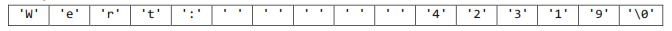
\includegraphics[width=0.6\textwidth]{pics/bsp1.png}
		\lstinputlisting[language=C,tabsize=2]{code/uint2strf.c}
	\subsection	{Russische Multiplikation}
		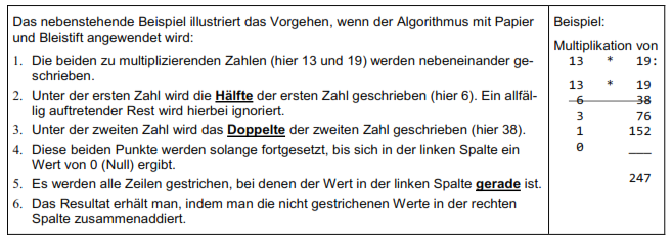
\includegraphics[width=0.6\textwidth]{pics/bsp2.png}
		\lstinputlisting[language=C,tabsize=2]{code/russMult.c}
		
		